\documentclass[nohyperref]{article}
\usepackage{microtype}
\usepackage{graphicx}
\usepackage{subfigure}
\usepackage{booktabs} % for professional tables

% hyperref makes hyperlinks in the resulting PDF.
% If your build breaks (sometimes temporarily if a hyperlink spans a page)
% please comment out the following usepackage line and replace
% \usepackage{icml2022} with \usepackage[nohyperref]{icml2022} above.
\usepackage{hyperref}

% Attempt to make hyperref and algorithmic work together better:
\newcommand{\theHalgorithm}{\arabic{algorithm}}

\usepackage[accepted]{icml2022}

% If accepted, instead use the following line for the camera-ready submission:
% \usepackage[accepted]{icml2022}

\usepackage{amsmath}
\usepackage{amssymb}
\usepackage{mathtools}
\usepackage{amsthm}
% if you use cleveref..
\usepackage[capitalize,noabbrev]{cleveref}
\theoremstyle{plain}
\newtheorem{theorem}{Theorem}[section]
\newtheorem{proposition}[theorem]{Proposition}
\newtheorem{lemma}[theorem]{Lemma}
\newtheorem{corollary}[theorem]{Corollary}
\theoremstyle{definition}
\newtheorem{definition}[theorem]{Definition}
\newtheorem{assumption}[theorem]{Assumption}
\theoremstyle{remark}
\newtheorem{remark}[theorem]{Remark}

% Todonotes is useful during development; simply uncomment the next line
%    and comment out the line below the next line to turn off comments
%\usepackage[disable,textsize=tiny]{todonotes}
\usepackage[textsize=tiny]{todonotes}

% The \icmltitle you define below is probably too long as a header.
% Therefore, a short form for the running title is supplied here:
% \icmltitlerunning{WebQA Team 6}

\begin{document}

    \twocolumn[
        \icmltitle{WebQA Dataset Analysis}

% It is OKAY to include author information, even for blind
% submissions: the style file will automatically remove it for you
% unless you've provided the [accepted] option to the icml2022
% package.

% List of affiliations: The first argument should be a (short)
% identifier you will use later to specify author affiliations
% Academic affiliations should list Department, University, City, Region, Country
% Industry affiliations should list Company, City, Region, Country

% You can specify symbols, otherwise they are numbered in order.
% Ideally, you should not use this facility. Affiliations will be numbered
% in order of appearance and this is the preferred way.
        \icmlsetsymbol{equal}{*}

        \begin{icmlauthorlist}
            \icmlauthor{Haofei Yu}{}
            \icmlauthor{Jiyang Tang}{}
            \icmlauthor{Ruiyi Wang}{}
            \icmlauthor{Ziang Zhou}{}
        \end{icmlauthorlist}

% \icmlaffiliation{cmu}{xxx}

        \icmlkeywords{Machine Learning, ICML}

        \vskip 0.3in
    ]

% this must go after the closing bracket ] following \twocolumn[ ...

% This command actually creates the footnote in the first column
% listing the affiliations and the copyright notice.
% The command takes one argument, which is text to display at the start of the footnote.
% The \icmlEqualContribution command is standard text for equal contribution.
% Remove it (just {}) if you do not need this facility.

%\printAffiliationsAndNotice{}  % leave blank if no need to mention equal contribution
%\printAffiliationsAndNotice{\icmlEqualContribution} % otherwise use the standard text.

%\begin{abstract}
%\end{abstract}


    \section{Statistical Analysis}\label{intro}

    WEBQA \cite{webqa} is a novel and challenging benchmark for multi-modal, multi-hop, open-domain question answering. Generally speaking, this dataset includes 36,766 training samples,  4,966 validation samples, and 7,540 test samples. Based on different annotation standards, the whole dataset can be classified into two types of data: image-based annotated samples and text-based annotated samples.

    The text-based questions are spread out across a large territory and it makes them hard to find a categorization method that would nicely summarize them into discrete buckets. The linguistic complexity of text-based annotated questions is also greater than that of image-based questions. As a result, text-based annotated samples are all classified as $\mathit{text}$ and have no fine-grained sub-classes. When it comes to the image-based questions, since these question-answer pairs are more straightforward and easy to answer, the dataset are classified into 6 different types: $\mathit{YesNo}$, $\mathit{choice}$, $\mathit{number}$, $\mathit{color}$, $\mathit{shape}$, $\mathit{Others}$. They are demonstrated in Figure.~\ref{fig:qcate_pie}

    \begin{figure}[h]
        \center
        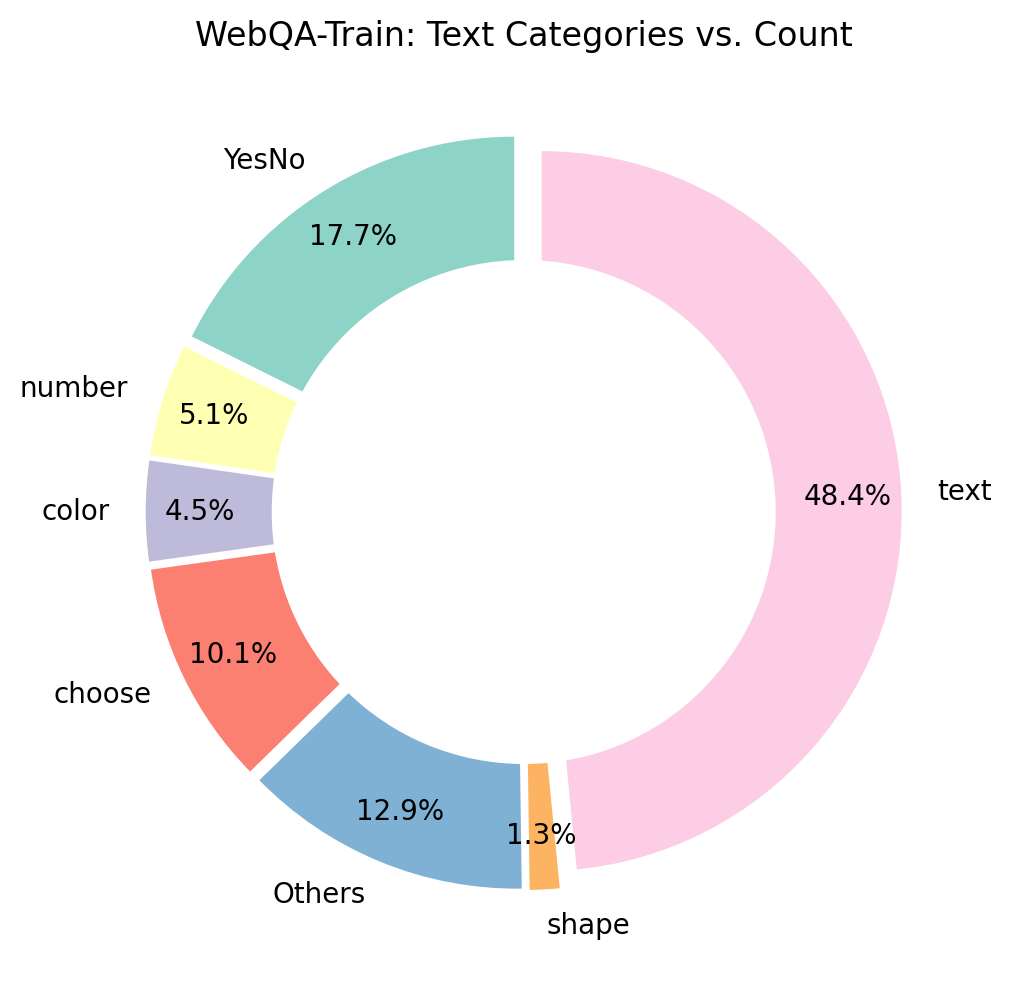
\includegraphics[width=0.4\textwidth]{img/train_textCat2count.png}
        \caption{Statistical information of Question Categories in Training Set}
        \label{fig:qcate_pie}
    \end{figure}


    More information with regard to question-answer pairs is provided in the WEBQA dataset. The first part of the additional information is the topic of the question-answer pairs. The second part of that is the negative text and image pairs. Concerning topic information, there are 433 different topics in the training dataset and 356 topics in the development dataset. Example topics are streets, plaza, american museum of natural history, etc. The distribution of topics in the training dataset is plotted in Figure.~\ref{fig:topic_distr}. Most of the topics, which include 348 topics, are overlapped between the training and development dataset. Only 401 samples in the training dataset own unique topics and only 9 samples in the development dataset have unique topics. Therefore, we can conclude that most topics for the data are shared between training and validation. It means that there is no out-of-distribution problem with regard to training and evaluation.
    \begin{figure}[h]
        \center
        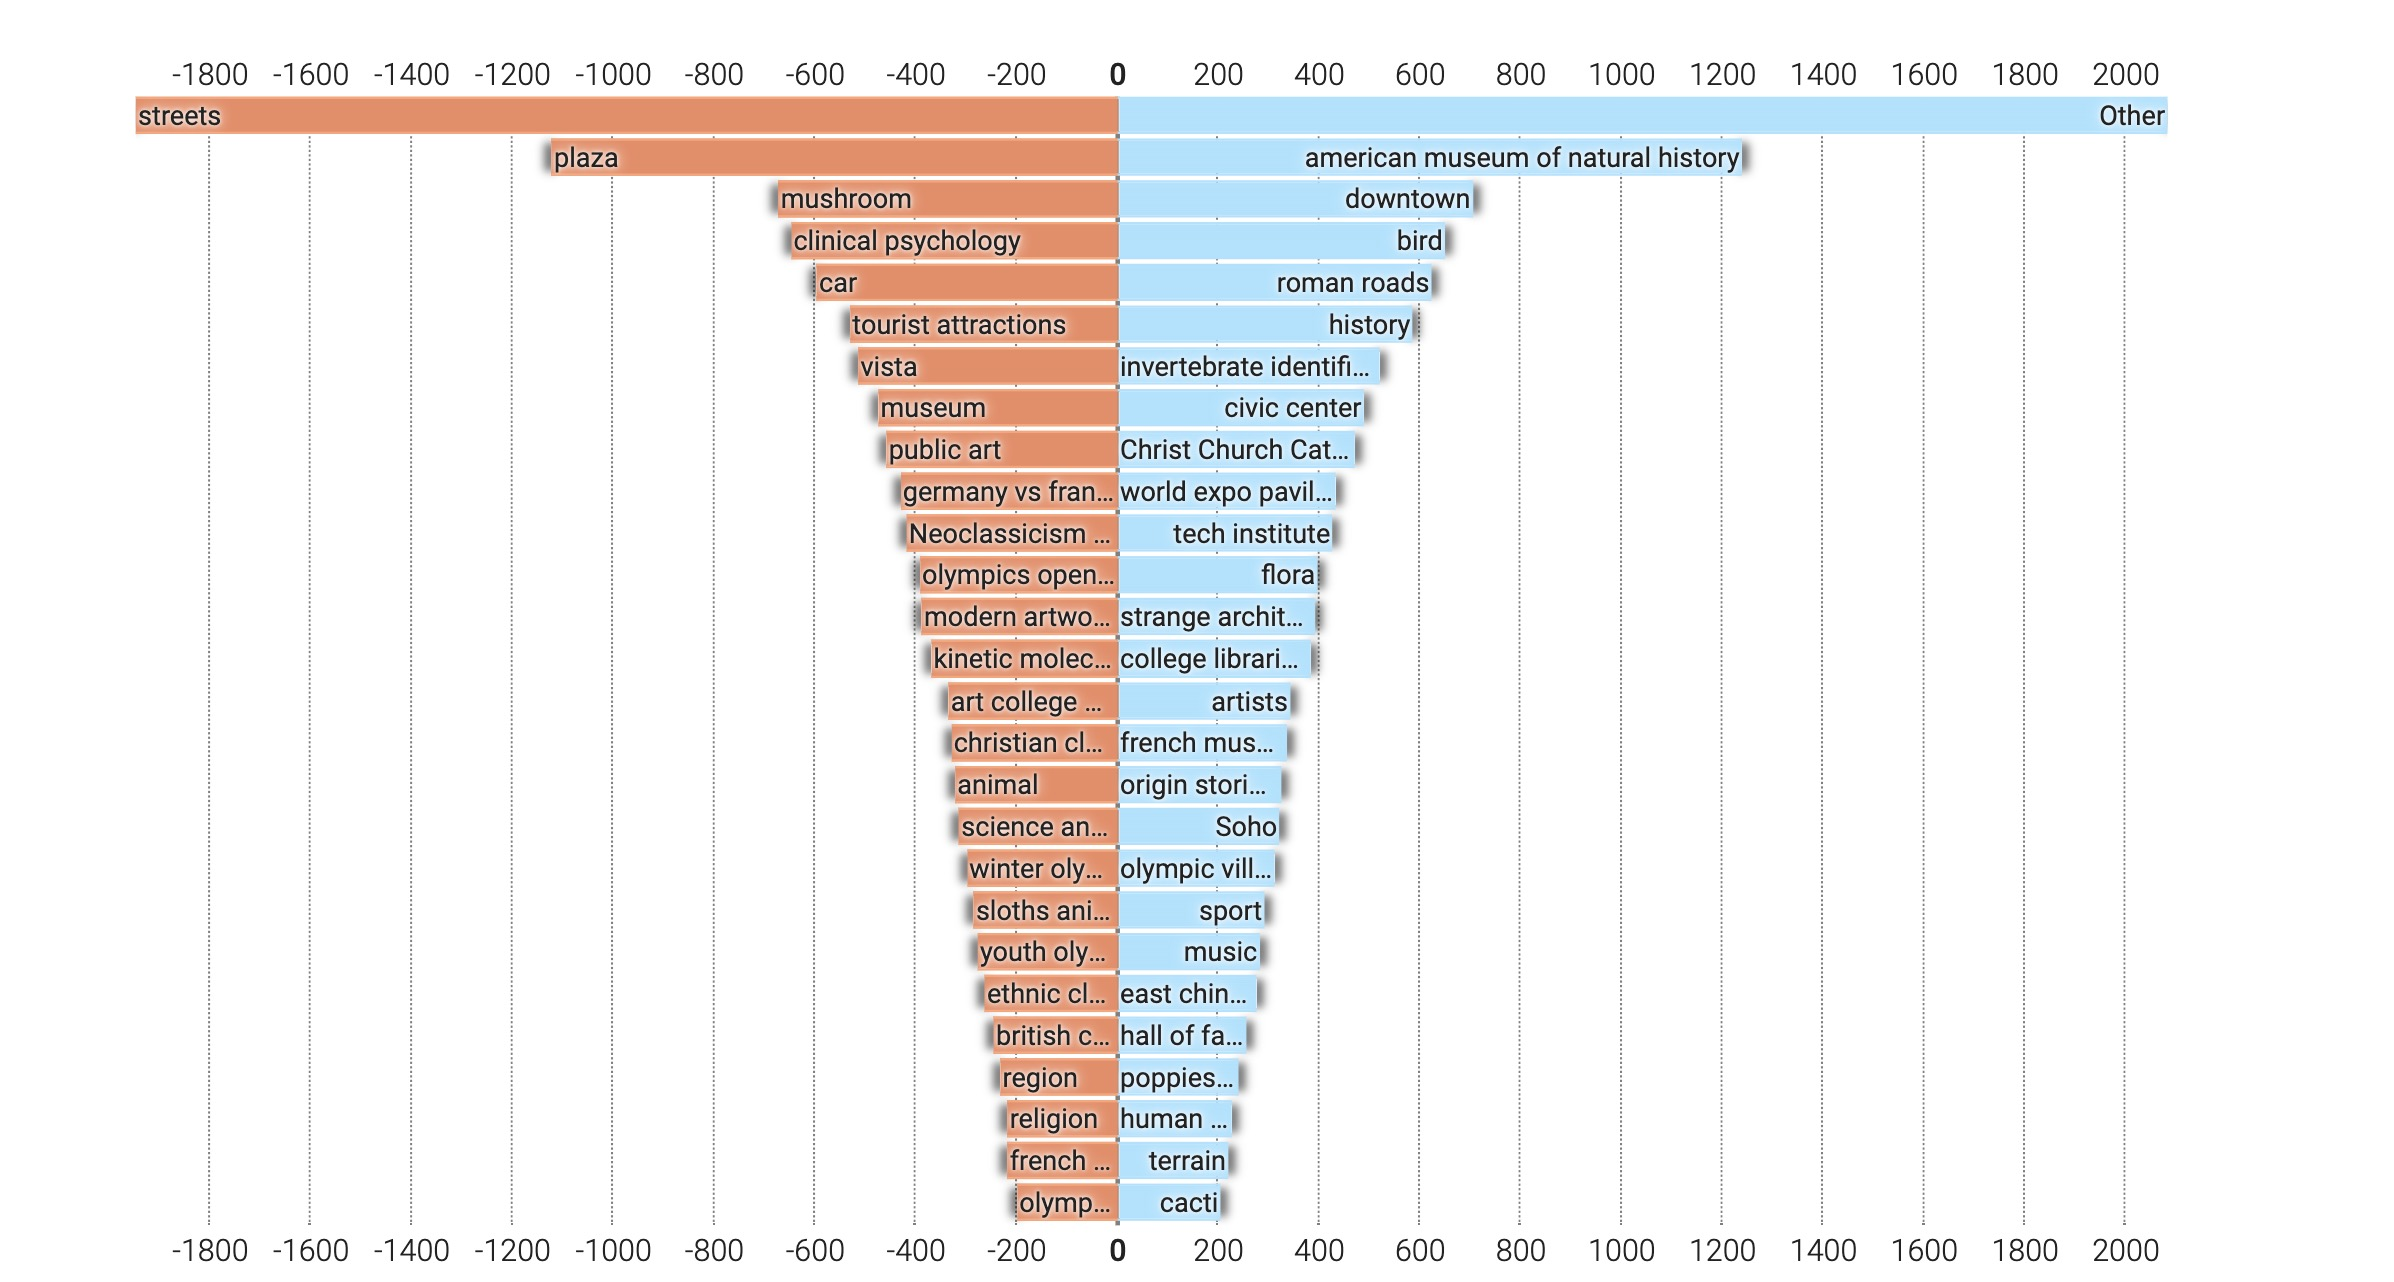
\includegraphics[width=0.55\textwidth]{img/topic_distribution.jpg}
        \caption{Distribution of topics of the training dataset}
        \label{fig:topic_distr}
    \end{figure}

    Another part of the additional information mentioned in the WEBQA dataset is both positive and negative image-based and text-based facts. The negatives in the dataset are hard in the sense that they have a large lexical overlap with the question but are not helpful for answering the questions. The positives are carefully checked during the initial annotation process and are ensured that false positives are not included. It is worth noticing that for image-based question-answering pairs, text positives are not provided while for text-based question-answering pairs, image positives are not provided. As a result, we calculate statistical information about positive samples and negative samples separately on image-based question-answering pairs and text-based question-answering pairs. Table \ref{tb:stat2} shows how many average positives and negatives belong to each sample in the dataset.



    \begin{table}[t]
        \centering
        \footnotesize
        \begin{tabular}{@{}l@{\hspace{4pt}}r@{\hspace{10pt}}r@{\hspace{10pt}}r@{\hspace{3pt}}r@{\hspace{10pt}}r@{\hspace{6pt}}r@{}}
            Train          & \#Img(+) & \#Img(-) & \#Txt(+) & \#Txt(-) \\
            \toprule
            Image-based QA & 1.44     & 15.85    & 0        & 15.35    \\
            \midrule
            Text-based QA  & 0        & 11.61    & 2.03     & 14.62    \\
            \midrule
            \midrule
            Dev            & \#Img(+) & \#Img(-) & \#Txt(+) & \#Txt(-) \\
            \toprule
            Image-based QA & 1.44     & 15.88    & 0        & 15.29    \\
            \midrule
            Text-based QA  & 0        & 11.78    & 2.04     & 14.63    \\
            \bottomrule
        \end{tabular}
        \caption{Statistical information about both image-based and text-based negatives and positives. Each number in this table represents the average number of text-based and image-based positives and negatives that one sample has.}
        \label{tb:stat2}
        \vspace{-5pt}
    \end{table}


    \section{Overlap Analysis}

    \begin{table}[t]
        \centering
        \footnotesize
        \begin{tabular}{@{}l@{\hspace{4pt}}r@{\hspace{10pt}}r@{\hspace{10pt}}r@{\hspace{3pt}}r@{\hspace{10pt}}r@{\hspace{6pt}}r@{}}
            Split & shape(\%) & YesNo(\%) & color(\%) \\
            \toprule
            Train & 92.67     & 66.54     & 99.33     \\
            \midrule
            Dev   & 95.95     & 68.24     & 97.21     \\
            \bottomrule
        \end{tabular}
        \caption{Domain set overlap information about $\mathit{YesNo}$, $\mathit{color}$, $\mathit{shape}$ types of questions and discuss whether ground-truth answers include corresponding domain set tokens which are used in the WEBQA final testing process.(domain set are specially designed token sets including \{Yes, No\} for $\mathit{YesNo}$ type, \{square, circle, ...\} for $\mathit{shape}$ type, \{golden, red, ...\} for $\mathit{color}$ type)}
        \label{tb:overlap1}
        \vspace{-5pt}
    \end{table}

    \citet{qa_overlap} mentions that 60-70\% of test-time answers are also present somewhere in the training sets in widely used open-domain question-answering datasets. Moreover, they find that 30\% of
    test-set questions have a near-duplicate paraphrase in their corresponding training sets. In this section, we follow this idea and analyze whether there is an answer or question overlap between the different splits of the dataset.

    As mentioned in Section1, WEBQA has different types of questions and their evaluation metrics are different based on their types. We consider their overlap analysis separately. For the first type, including question types of $\mathit{YesNo}$, $\mathit{number}$, $\mathit{color}$, $\mathit{shape}$, WEBQA uses the F1 results calculated from intersected keywords and generated tokens as evaluation metrics. The intersected keywords are made from domain set keywords and ground-truth test keywords in the test set. Since this type of question has typical answering scopes, we can use the provided domain set and calculate its coverage on the training dataset and development dataset. Since $\mathit{number}$ type keywords is not provided, we leave this part of question-answering pairs to be future work. Table \ref{tb:overlap1} shows that there are still relatively some samples that have no words related in the domain sets.

    The evaluation script provided by the WebQA dataset calculates the accuracy and F1 score based on the number of intersections between true answers and the domain set and the number of intersections between predicted answers and the domain set. Take an example of the $\mathit{YesNo}$ question type, where the domain set is just \{Yes, No\}. There are more than $30\%$ answers of the training and development dataset that do not contain the keywords ``yes'' or ``no''. Given the official evaluation script, all the predicted answers under such cases are marked as wrong. To further investigate the real accuracy of those cases in the $\mathit{YesNo}$ question type where the true answers are not related to the domain set, we manually labeled the correctness of the answers produced by the baseline models with respect to the development dataset.

    The number of out-of-domain answers in the development is 263, and we randomly sampled 50 pairs from the validation outputs from both the vinvl and x101fpn baseline models that are marked as incorrect. Table \ref{tb:acc_result} shows that the real accuracy in both baseline models is fairly high, indicating that those cases falling out of the domain set are dragging down the actual accuracy of the model. For future work, we need to find a better way to evaluate the accuracy of the out-of-domain cases instead of just finding the intersections of the domain set.

    \begin{table}[h]
        \centering
        \footnotesize
        \begin{tabular}{@{}l@{\hspace{4pt}}r@{\hspace{10pt}}r@{\hspace{10pt}}r@{\hspace{3pt}}r@{\hspace{10pt}}r@{\hspace{6pt}}r@{}}
            Baseline Model & vinvl & x101fpn \\
            \toprule
            Accuracy       & 82\%  & 82\%    \\
            \midrule
            \# Samples     & 50    & 50      \\
            \bottomrule
        \end{tabular}
        \caption{Manually calculated accuracy of 50 randomly selected samples of the vinvl and x101fpn baseline models where the real answers have no intersection with the $\mathit{YesNo}$ domain set.}
        \label{tb:acc_result}
        \vspace{-5pt}
    \end{table}

    For the second type, including question types of $\mathit{choice}$, $\mathit{Others}$, and $\mathit{text}$, WEBQA uses the recall calculated from test keywords and generated tokens as evaluation metrics. Since the test keywords are not publicly available, we utilize $\mathit{noun\_chunks}$ API in the $\mathit{spaCy}$ to analyze the noun overlap between the development dataset and training dataset. Table \ref{tb:overlap2} shows that more than 30\% of nouns mentioned in the questions or answers in the dev/test dataset actually have appeared in the training dataset before. As a result, it is one of the potential points for model improvement.


    \begin{table}[h]
        \centering
        \footnotesize
        \begin{tabular}{@{}l@{\hspace{4pt}}r@{\hspace{10pt}}r@{\hspace{10pt}}r@{\hspace{3pt}}r@{\hspace{10pt}}r@{\hspace{6pt}}r@{}}
            & \#train & \#dev  & \#shared & overlap(\%) \\
            \toprule
            Questions & 53,469  & 9,793  & 3,736    & 38.14       \\
            \midrule
            Answers   & 31,224  & 5,367  & 1,895    & 35.31       \\
            \midrule
            \midrule
            & \#train & \#test & \#shared & overlap(\%) \\
            \toprule
            Questions & 53,469  & 20,787 & 6,290    & 30.26       \\
            \bottomrule
        \end{tabular}
        \caption{Noun overlap information in answers and questions between training dataset and development dataset. Each number in the table represents the unique noun number in the splits of dataset. Only $\mathit{choice}$, $\mathit{Others}$ , and $\mathit{text}$ samples are taken into consideration in this table. Overlap ratio is calculated by dividing number of shared nouns with total number of nouns in the dev/test dataset.}
        \label{tb:overlap2}
        \vspace{-5pt}
    \end{table}


    \section{Fact Analysis}

    \begin{table*}[ht]
        \centering
        \footnotesize
        \begin{tabular}{@{}l@{\hspace{4pt}}r@{\hspace{10pt}}r@{\hspace{10pt}}r@{\hspace{10pt}}r@{\hspace{10pt}}r@{\hspace{10pt}}r@{}}
            Positiveness   & \#PosFacts & \#NegFacts &         &         &          &          \\
            \toprule
            Train          & 2,658      & 3,673      &         &         &          &          \\
            Dev            & 561        & 1,343      &         &         &          &          \\
            Test           & 1,216      & 1,732      &         &         &          &          \\
            \midrule
            \midrule
            Question Types & \#YesNo    & \#number   & \#color & \#shape & \#choose & \#Others \\
            \midrule
            Train          & 369        & 95         & 75      & 28      & 168      & 265      \\
            Dev            & 142        & 57         & 40      & 18      & 111      & 132      \\
            Test           & 597        & 227        & 160     & 49      & 438      & 529      \\
            \bottomrule
        \end{tabular}
        \caption{Statistics of the image classification subset in terms of positiveness and question types}
        \label{tab:image_classification_subset}
        \vspace{-5pt}
    \end{table*}


    As mentioned in \cite{webqa}, questions can contain one or two positive image facts and several negative ones.
    The input of the VLP model is the prediction result of a pretrained faster RCNN \cite{faster-rcnn} on such images.
    More specifically, the output of the faster RCNN model's last layer, the bounding
    box coordinates, the object class labels, and the confidence scores are used.

    \begin{figure}[ht]
        \center
        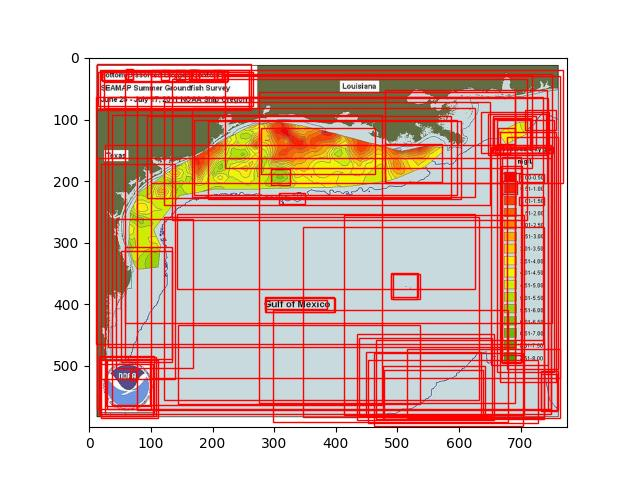
\includegraphics[width=0.45\textwidth]{img/rcnn-box}
        \caption{The bounding boxes produced by RCNN}
        \label{fig:rcnn-bounding-boxes}
    \end{figure}

    Figure \ref{fig:rcnn-bounding-boxes} shows an example image and the bounding boxes produced by the RCNN model.
    Note that there are a large number of bounding boxes, some of them even overlapping, because
    the RCNN model was trained on visual genome dataset which contains detailed descriptions for objects, their
    attributes, and relationships \cite{visualgenome}.
    This is ideal for WebQA because we want the VLP model to be aware of as many details about the images as possible.

    The negative image facts are obtained using hard negative mining.
    However, \cite{webqa} didn't mention the detailed procedure of this process.
    We obtained more details from the authors.
    During the initial annotation process, each annotator was provided with a set of evidences and
    they selected some of them to create a question that can be answered by these evidences.
    The unselected evidences naturally became negative facts.
    In addition, the authors have a retrieval baseline that selects evidences based on their captions' lexical overlap
    with the question, and the samples that deceived this baseline became additional hard negatives.
    Finally, the authors manually validated these hard negatives to ensure there is no false positive.

    Intuitively, human first read the question and then select which images to use as positive samples based on the
    question content.
    That means the hard negatives must be difficult to be distinguished from the positives for the VLP model
    without seeing the question.
    Therefore, we want to verify this assumption by analyzing the image facts without the questions.

    \subsection{Image Embedding Visualization}

    We treat the output of the RCNN model's final layer as the image embeddings, and visualized them with regard to
    positiveness and question type using PCA dimension reduction, as shown in Figure \ref{fig:rcnn_embed_vs_pos_neg} and
    Figure \ref{fig:rcnn_embed_vs_qcate}.

    \begin{figure}[h]
        \center
        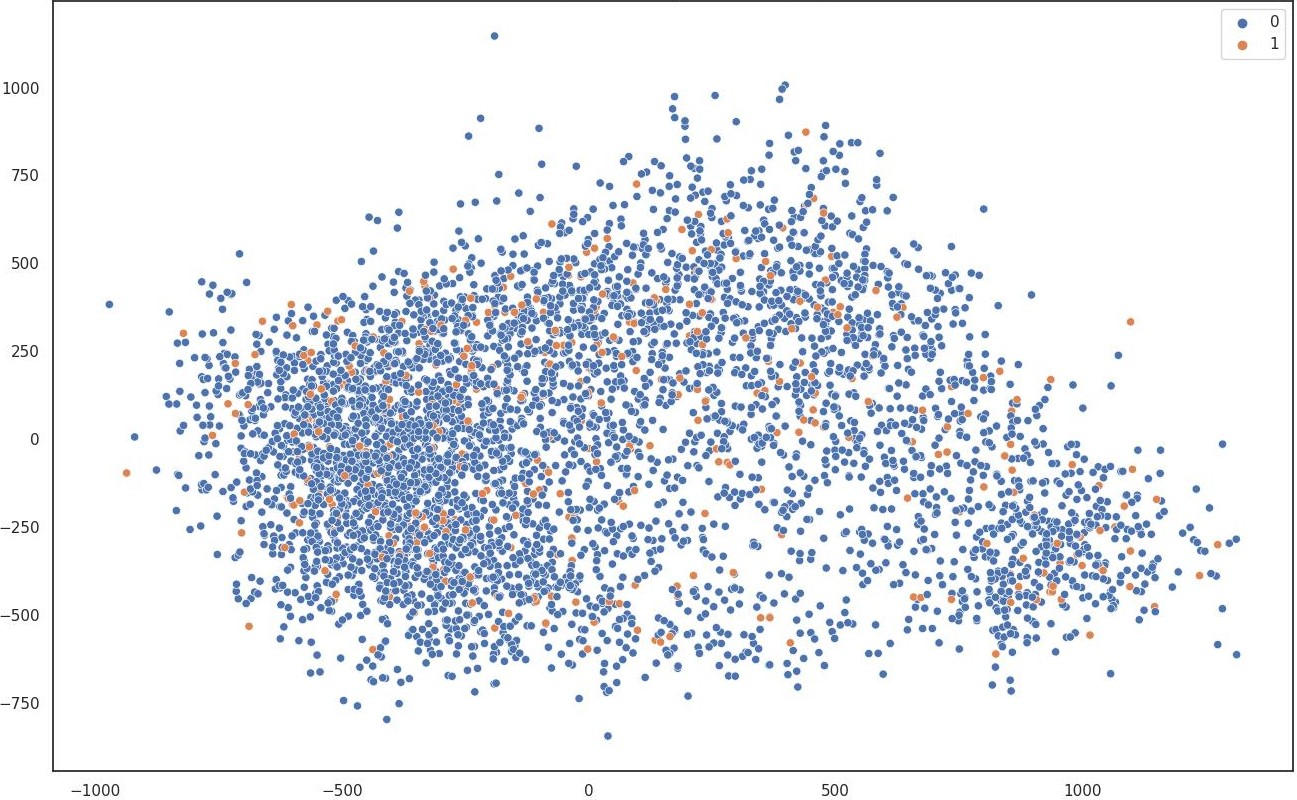
\includegraphics[width=0.45\textwidth]{img/rcnn_embed_vs_pos_neg.jpg}
        \caption{The PCA of RCNN embeddings vs. positiveness}
        \label{fig:rcnn_embed_vs_pos_neg}
    \end{figure}

    \begin{figure}[h]
        \center
        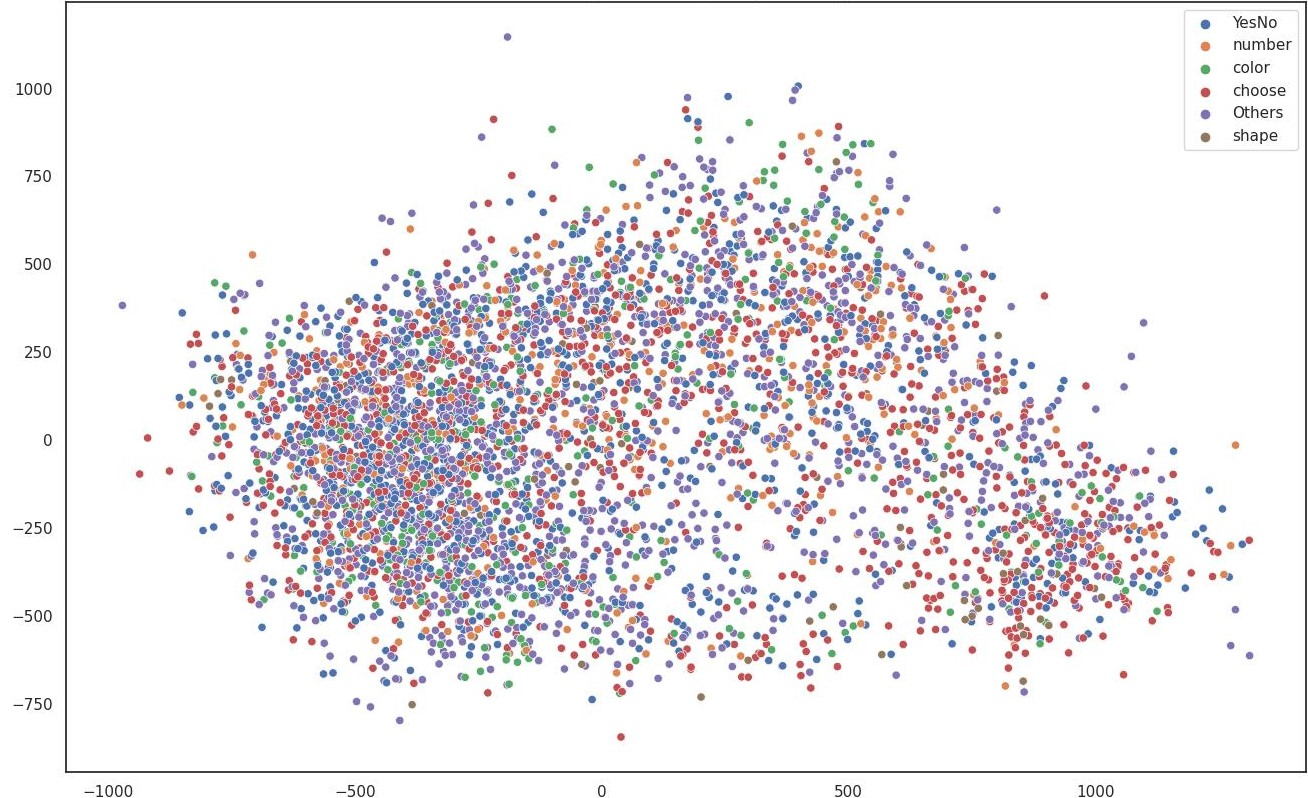
\includegraphics[width=0.45\textwidth]{img/rcnn_embed_vs_qcate.jpg}
        \caption{The PCA of RCNN embeddings vs. question types}
        \label{fig:rcnn_embed_vs_qcate}
    \end{figure}

    \subsection{Text Embedding Visualization}
    In \cite{webqa}, the authors used \text{Bert-base-cased} model as tokenizer to obtain the textual embeddings of textual sources and image captions. Rather that having multiple embeddings in each sentence, in this analysis, we used sentence transformers \cite{sbert} directly to extract utterance-level embeddings for simplicity and intuitiveness. Each token in a sentence will be represented by a 384-dimension vector, and the embedding of each sentence is by taking average of all token embeddings. The samples choices are aligned with the selected images. Following the same PCA settings, we visualize the reduced textual embeddings in Figure.~\ref{fig:text_train_posneg_pca} and Figure.~\ref{fig:text_train_qcate_pca}, hoping to verify our assumptions.

    \begin{figure}[h]
        \center
        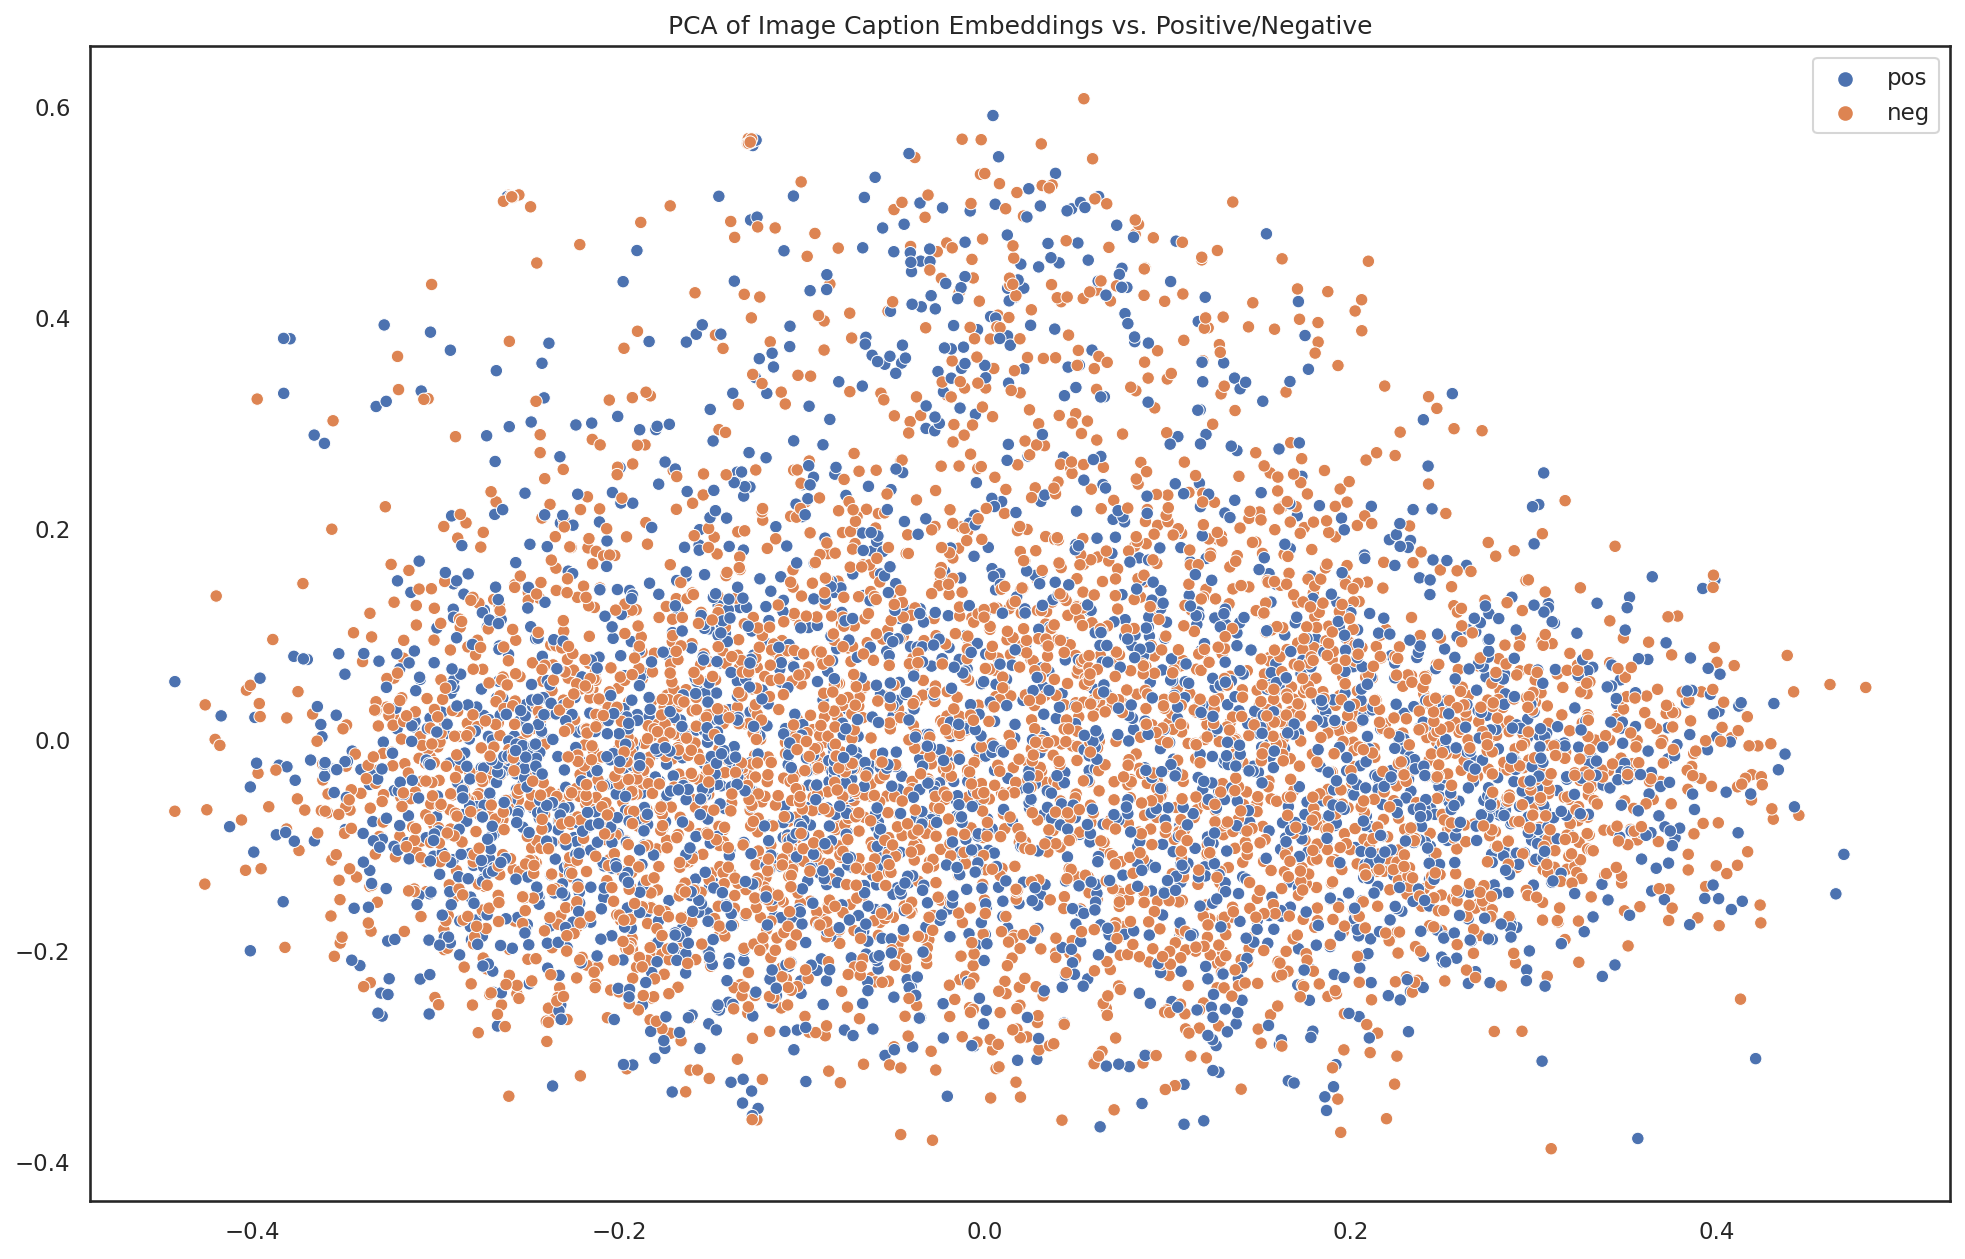
\includegraphics[width=0.45\textwidth]{img/text_train_posneg_pca.png}
        \caption{The PCA of Image Caption Embeddings vs. positiveness}
        \label{fig:text_train_posneg_pca}
    \end{figure}

    \begin{figure}[h]
        \center
        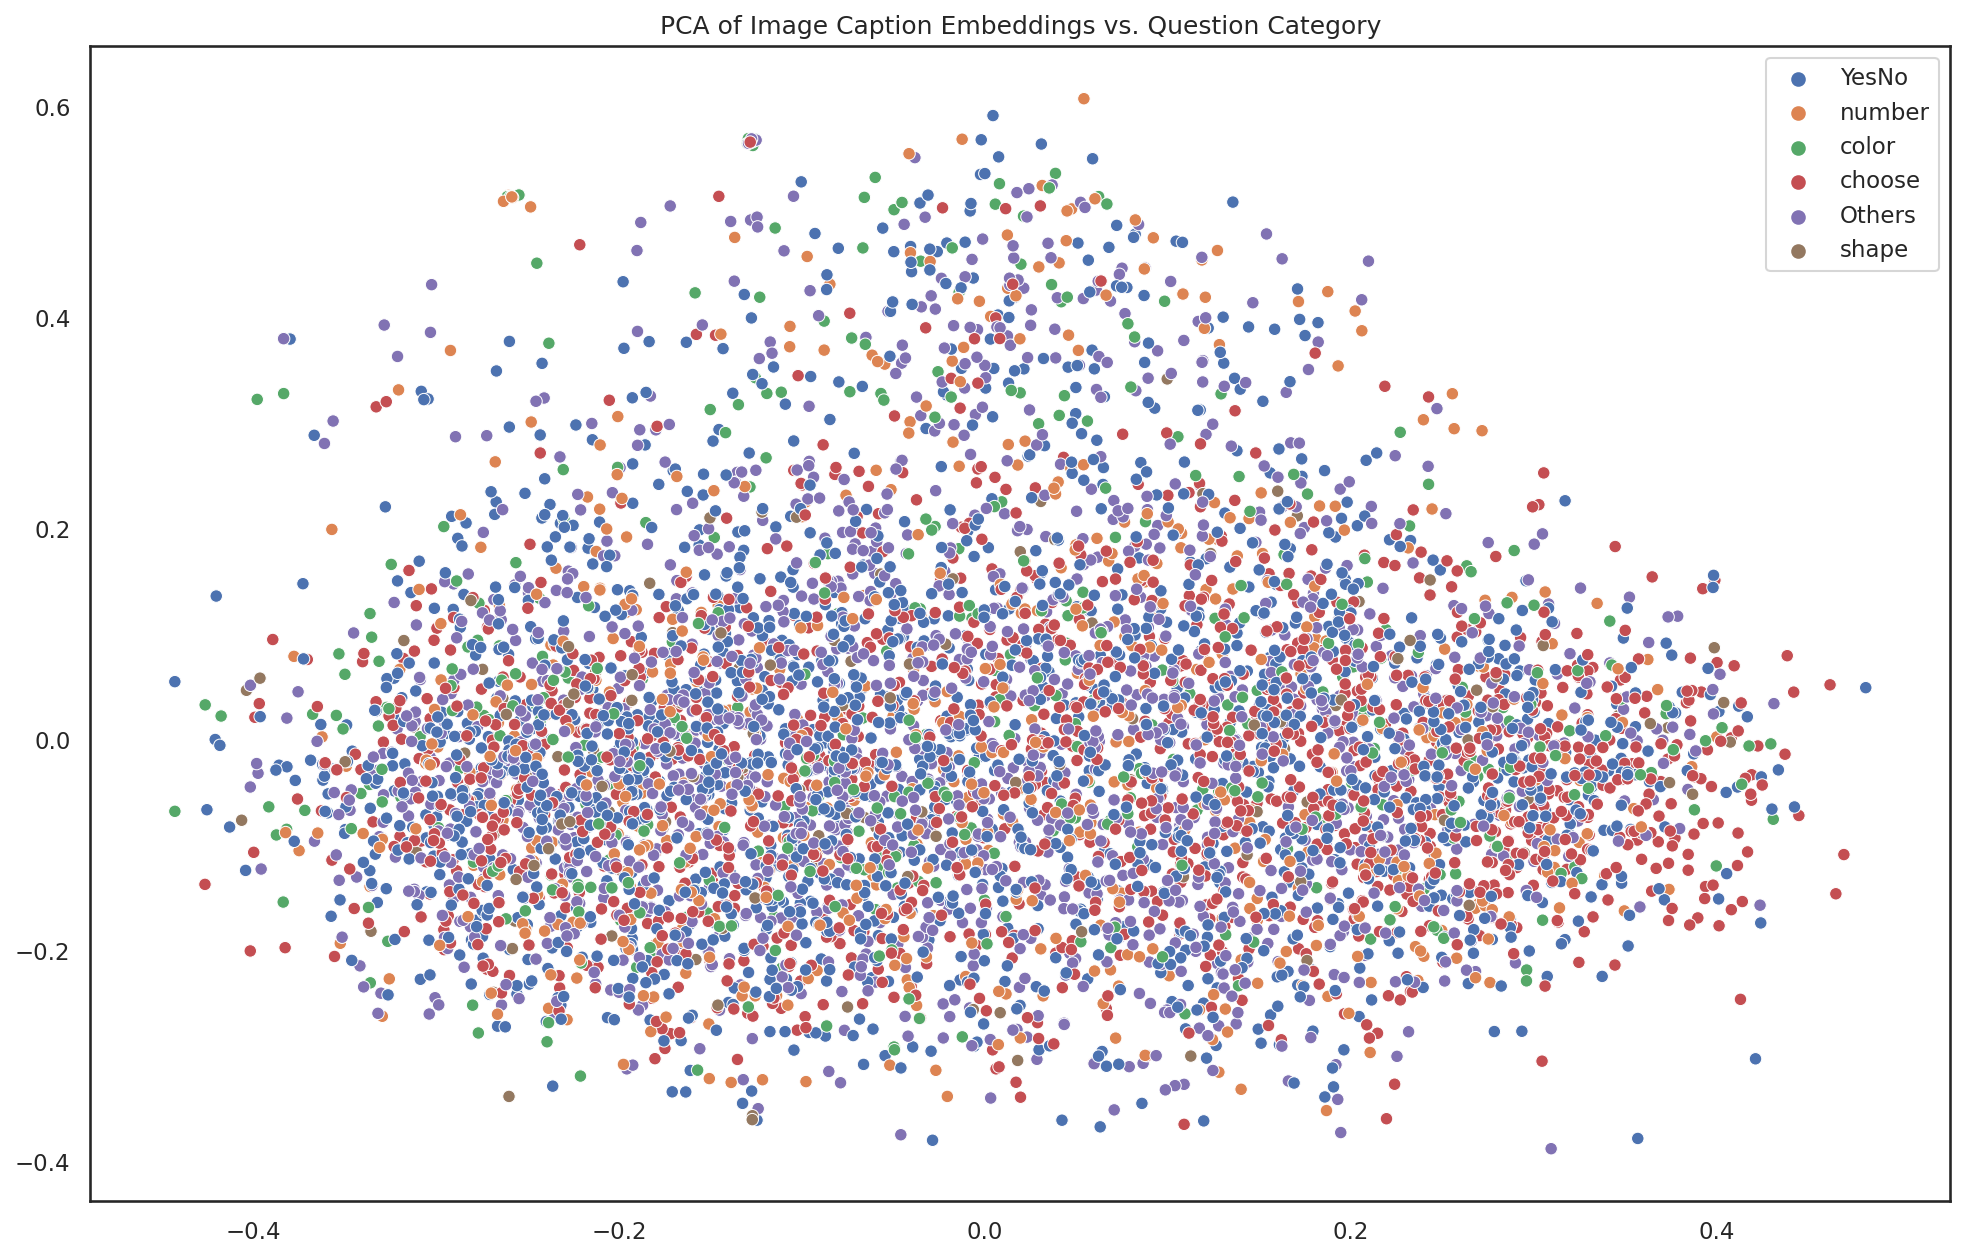
\includegraphics[width=0.45\textwidth]{img/text_train_qcate_pca.png}
        \caption{The PCA of Image Caption Embeddings vs. Question Categories}
        \label{fig:text_train_qcate_pca}
    \end{figure}

    As shown from Figure.~\ref{fig:rcnn_embed_vs_pos_neg} to Figure.~\ref{fig:text_train_qcate_pca}, there's no apparent pattern or clusters in regard to question types or fact positiveness.
    This gives us a rough impression that the images or image captions alone contain insufficient information to infer their question
    types and fact positiveness.
    However, this doesn't necessarily verify our assumption, because
    \begin{itemize}
        \item there could be some patterns in data that cannot be seen from PCA visualization,
        \item and the RCNN embeddings do not comprehensively represent the images.
    \end{itemize}

    Therefore, to properly verify our assumption, we need to perform some classification experiments on raw image input.

    \subsection{Image Classification Experiments}

    We extracted a subset from WebQA that has a balanced number of positive and negative facts.
    See Table \ref{tab:image_classification_subset} for the statistics of the subset.
    In addition, there are 74 question topics in this subset.

    We first need a baseline experiment to prove that our classifier indeed has the capability of
    distinguishing different types of images.
    Therefore, a topic classifier is trained.
    Then, two more classifiers are trained, one for predicting question types and the other for predicting fact
    positiveness.
    We expect the topic classifier to show some classification capability and
    the other two two classifiers to diverge during the training process or to perform badly on the test data.

    The classifiers share the same structure, a ResNet50 \cite{resnet} trained on ImageNet dataset \cite{imagenet}
    followed by a linear output layer.
    They are finetuned on the image subset for 15 epochs.

    The results shown in Table \ref{tab:image_classification_results} indeed meet our expectation.
    The topic classifier shows some classification capability in terms of accuracy and F1 score on classifying 74 topics.
    However, the question type and positiveness classifier failed to even converge.
    And their classification performance is no better than random guesses.

    \begin{table}[ht]
        \centering
        \footnotesize
        \begin{tabular}{@{}l@{\hspace{4pt}}r@{\hspace{10pt}}r@{\hspace{10pt}}r@{\hspace{10pt}}r@{\hspace{10pt}}r@{\hspace{10pt}}r@{}}
            & Accuracy & F1 Score & Precision & Recall \\
            \toprule
            \midrule
            Topic         & 0.32     & 0.35     & 0.35      & 0.40   \\
            \midrule
            Question Type & 0.33     & 0.19     & 0.20      & 0.21   \\
            \midrule
            Positiveness  & 0.55     & 0.50     & 0.51      & 0.51   \\
            \bottomrule
        \end{tabular}
        \caption{Image classification model performance on test set}
        \label{tab:image_classification_results}
        \vspace{-5pt}
    \end{table}

    In conclusion, we believe that the image negatives cannot be distinguished from the positives without seeing the
    questions.



    \clearpage

    \bibliography{main}
    \bibliographystyle{icml2022}

\end{document}
